\documentclass{article}
\usepackage{amsmath}
\usepackage{tikz}
\usepackage[utf8]{inputenc}
\usepackage{float}

\usetikzlibrary{shapes ,arrows}


\title{TP N$^\circ$1 \\ Sistemas controlados por computadora}
\author{Saez, Lautaro Andres}
\date{}



\begin{document}
    \maketitle
  

    \tikzstyle{block} = [draw, fill=blue!20, rectangle, 
    minimum height=3em, minimum width=6em]
    \tikzstyle{sum} = [draw, fill=blue!20, circle, node distance=1cm]
    \tikzstyle{input} = [coordinate]
    \tikzstyle{output} = [coordinate]
    \tikzstyle{pinstyle} = [pin edge={to-,thin,black}]
    \tikzstyle{big-block} = [draw, rectangle, minimum height= 12em, minimum width= 24em]

    \section{Ejercicio 1}

        El proceso que se modela esta descripto por 

        \begin{equation}
            G(s) = \frac{1}{( s + 0.2 )( s + 0.3 )( s + 0.5 )}
        \end{equation}
        
        \begin{figure}[!htb]
            \centering
            \begin{tikzpicture}[node distance=2.5cm,auto,>=latex']
                \node [input, name=input] {};
                \node [sum, right of=input] (sum) {$+$};
                \node [block, right of=sum] (controller) {$G_c(s)$};
                \node [block, right of =controller, node distance=3.5cm] (system) { $\frac{1}{( s + 0.2 )( s + 0.3 )( s + 0.5 )}$ };

                \draw [->] (controller) -- node[name=u] { $u$ } (system);
                \node [output, right of=system] (output) {};
                \node [output, below of=u] (H) {};
                
                \draw [draw, ->] (input) -- node {$r$} (sum); 
                \draw [->] (sum) -- node {$e$} (controller);
                \draw [->] (system) -- node[name=y] {$y$} (output);
                \draw [-] (y) |- (H);    
                \draw [->] (H) -| node[pos=0.99] {$-$} (sum);

            \end{tikzpicture}
            \caption{Sistema retroalimentado}
            \label{fig:sys-retro}
        \end{figure}
        


        \subsection{a)}

        Para calcular el error en estado estacionario una forma es encontrar la transferencia entre el error $E(s)$ y la referencia $R(s)$. Es posible expresar 

        \begin{equation}
            E(s) = R(s) - Y(s)
        \end{equation}

        De esta forma se obtiene que 

        \begin{equation}
            E(s) = \frac{1}{( s + 0.2 )( s + 0.3 )( s + 0.5 ) + G_c(s)} R(s)
        \end{equation}

        Para cualquier controlador, si colocamos un proporcional, es decir $G_c(s)=k_c$

        \begin{equation}
            E(s) = \frac{1}{( s + 0.2 )( s + 0.3 )( s + 0.5 ) + k_c} R(s)
        \end{equation}

        El error en estado estacionario se calcula como 

        \begin{equation}
            \lim_{t \to \infty} e(t) = \lim_{s \to 0} s E(s)
        \end{equation}

        Si la entrada de referencia es un escalon tenemos que 

        \begin{equation}
            \lim_{s \to 0} \frac{s}{( s + 0.2 )( s + 0.3 )( s + 0.5 ) + k_c} \frac{1}{s} = \frac{1}{(0.2)0.3)(0.5) + k_c}
        \end{equation}

        Por lo tanto el error en estado estacionaro queda definido como 

        \begin{equation}
            e_\infty = \frac{3}{3 + 100k_c}
        \end{equation}

        \begin{figure}[!htb]
            \centering
            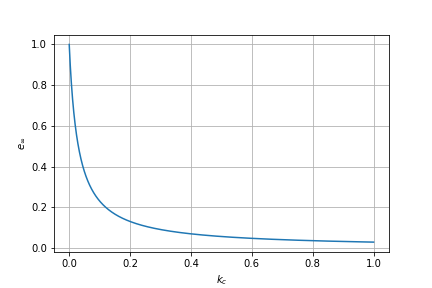
\includegraphics[width=\textwidth]{Img/1-a.png}
            \caption{Grafico del error en función de $k_c$.}
            \label{}
        \end{figure}

        De la figura anterior se observa que el error decae de forma exponencial con el valor de $k_c$, asi que 
        en teoría lo óptimo seria colocar un valor de $k_c$ lo mas grande posible, aunque debemos analizar que sucedería
        con la estabilidad del sistema.



        \subsection{b)}

    Para ajustar un \textbf{PID} por el segundo criterio de Z-Nichols en primera instancia debemos calcular la 
    $k_c$ maxima y luego la frecuencia critica del sistema.

    \subsubsection{$k_{c, max}$}

    El polinomio caracteristico del sistema retroalimentado con un proporcional que se obtiene es 

    \begin{equation}
        P(s) = s^3 + s^2 + 0.31s + 0.03 + k_c
    \end{equation}

    Una forma de obtener el $k_c$ maximo seria plantear las raices del sistema y analizar cuando sus polos son complejos puros, 
    otra forma seria tomar $s=j\omega$ y buscar el $k_c$ de tal manera de obtener dos raices complejas conjugadas. Por 
    ultimo podriamos plantear el criterio de estabilidad de Routh.

    \begin{table}
        \centering
        \begin{tabular}{|c|c|c|c|}
            \hline $s^3$ & $1$ & $0.31$ & $0$ \\
            \hline $s^2$ & $1$ & $0.03 + k_c$ & $0$ \\
            \hline $s$ & $0.28-k_c$ & $0$ & $0$ \\
            \hline $s^0$ & $0.03+k_c$ & $0$ & $0$ \\
            \hline
        \end{tabular}
    \end{table}

    Recordemos que para que se cumpla el criterio de estabilidad de Routh tanto la primer columna como todos los coeficientes del polinomio 
    caracteristico tienen que ser mayores a $0$, con lo que se obtiene 

    \begin{eqnarray}
        0.03 + k_c > 0 \land 0.28 - k_c > 0
    \end{eqnarray}

    De resolver estas inecuaciones se obtiene que $k_c \in [ -0.03 ; 0.28 ]$. Por lo tanto el $k_c$ maximo es $0.28$.

    \subsubsection{$\omega_{c}$}

    Para calcular $\omega_c$ debemos pedir que el argunmento del sistema sea $-180^\circ$, por lo tanto tenemos 

    \begin{eqnarray}
        \arg{ G_p(s) } = -180^\circ
    \end{eqnarray}

    Teniendo en cuenta que el sistema no tiene ceros y solo posee polos, la expresion que se obtiene es 

    \begin{eqnarray}
        -\arg\{ (j\omega)^3 + (j\omega)^2 + 0.31(j\omega) + 0.03  \} = -180^\circ
    \end{eqnarray}

    Por lo tanto 

    \begin{eqnarray}
        \frac{(0.31 - \omega^2)\omega}{0.03 - \omega^2} = 0
    \end{eqnarray}

    Lo cual simplifica el problema 

    \begin{eqnarray}
        0.31 - \omega^2 = 0
    \end{eqnarray}

    Por lo que se tiene que $\omega_c=0.56 r/s$.

    Utilizando las ecuacion de Z-Nichols 

    \begin{table}[!htb]
        \centering
        \begin{tabular}{|c|c|c|}
            \hline $k_c$ & $T_i$ & $T_d$ \\
            \hline $0.17$ & $\frac{25}{14} \pi$ & $\frac{25}{56} \pi$ \\
            \hline
        \end{tabular}
    \end{table}


        \subsection{c)}

        Para aplicar el método de margen de fase, es necesario definir nuestra frecuencia de cruce. Es usual tomar el 
        valor de la frecuencia de corte del sistema sin controlar. Por lo tanto 

        \begin{equation}
            \omega_{x} = \omega_{c, planta}
        \end{equation}

        Luego sabemos que el angulo en $\omega_x$ del lazo directo lo podemos calcular como 

        \begin{equation}
            \arg\{ G_c(j\omega_x)  \} + \arg\{ G( j\omega_x )  \} = -180^\circ + MF
        \end{equation}

        Dado que para este problema el $MF=30^\circ$ y $\arg\{ G( j\omega_x )  \}=-180^\circ$ entonces

        \begin{equation}
            \arg\{ G_c(j\omega_x)  \} = 30^\circ = \theta
        \end{equation}

        Luego podemos establecer las siguientes relaciones 

        \begin{equation}
            k_c = \frac{\cos \theta}{ | G(j\omega_x) | } \land k_c\left( T_d \omega_x - \frac{1}{T_i \omega_x} \right) = \frac{\sin \theta}{| G(j\omega_x) |}
        \end{equation}

        Una relación muy usual es plantear $T_i = 4T_d$, la misma que utiliza el método de Z-Nichols. En este caso obtenemos 

        \begin{equation}
            k_c = 0.25 \land T_i = 6.08 \land T_d = 1.52
        \end{equation}

        \subsection{d)}

        Primero debemos obtener que el margen de ganancia sea 2, por lo tanto $k_c|G(\omega_c)|=\frac{1}{2}$ como
        $|G(\omega_c)|\approx3.54$ entonces tomaremos $k_c=0.14$.
        
        Luego plantearemos que el PI no aporte mas de $5^\circ$ en la frecuencia critica, en este caso utilizaremos $3^\circ$, entonces:

        \begin{equation}
            \arg{ T_i\omega_cj +1 } - 90^\circ = 87^\circ \Leftrightarrow T_i = 34
        \end{equation}


    \section{Ejercicio 2}

        En este ejercicio se tiene la siguiente transferencia 

        \begin{equation}
            G(s) = \frac{1}{(s+1)(s-1)}
        \end{equation}

        Un sistema claramente inestable.

        \subsection{P}

        Si deseamos ajustar un proporcional, tenemos el lugar de las raices de la figura \ref{fig:2-P}.

        \begin{figure}[!htb]
            \centering
            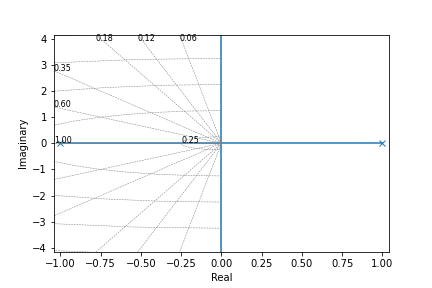
\includegraphics[width=.4\textwidth]{Img/2-P.png}
            \caption{Lugar de las raices para un control P.}
            \label{fig:2-P}
        \end{figure}

        \subsection{PI}

        Para este caso el lugar de las raices obtenido se puede observa en la figura \ref{fig:2-PI}, por lo tanto no 
        podemos controlar el sistema con un controlador PI.

        \begin{figure}[!htb]
            \centering
            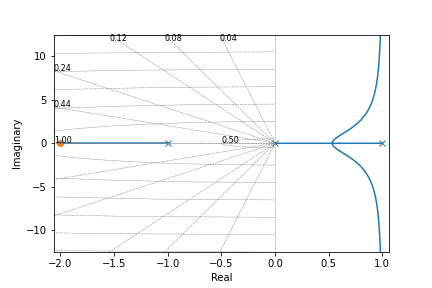
\includegraphics[width=.5\textwidth]{Img/2-PI.png}
            \caption{Lugar de las raices para un controlador PI con $T_i=1/2$.}
            \label{fig:2-PI}
        \end{figure}

        \subsection{PD}

        Para un controlador PD es posible controlar el sistema ya que no se agrega un polo en cero, ademas nos permite 
        volver todo lo rapido que queramos. El lugar de las raices lo podemos observar en la figura \ref{fig:2-PD}

        \begin{figure}[!htb]
            \centering
            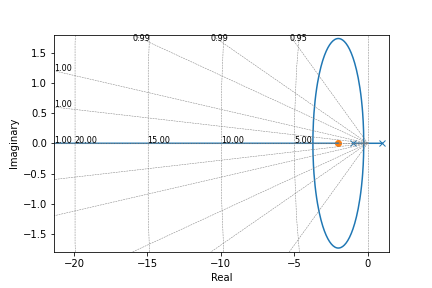
\includegraphics[width=.5\textwidth]{Img/2-PD.png}
            \caption{Lugar de las raices para un controlador PD con $T_d=1/2$.}
            \label{fig:2-PD}
        \end{figure}

        \subsection{PID}

        Con el PID es posible controlar el sistema pero es mas dificil de ajustar y la unica ventaja que obtenemos es el error 
        nulo en estado estacionario, el lugar de las raices lo observamos en la figura \ref{fig:2-PID}.

        \begin{figure}[!htb]
            \centering
            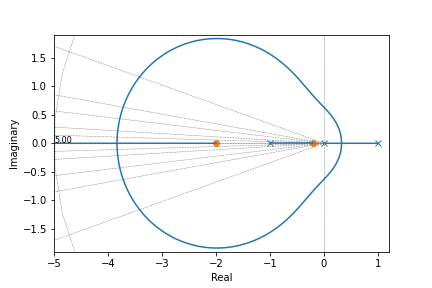
\includegraphics[width=.5\textwidth]{Img/2-PID.png}
            \caption{Lugar de las raices con un PID para $T_d=1/2$ y $T_i=5$.}
            \label{fig:2-PID}
        \end{figure}

        \subsection{Ajustando el controlador}

        Por simplicidad se decidio ajustar un PD, ya que solo debemos calcular $k_c$ para un $T_d$ definido. Se toma $T_d=1/2$, 
        por lo que la transferencia $H(s)$ queda definida como

        \begin{figure}[!htb]
            \centering
            \begin{tikzpicture}[node distance=2.5cm,auto,>=latex']
                \node [input, name=input] {};
                \node [sum, right of=input] (sum) {$+$};
                \node [block, right of=sum] (controller) {$k_c ( 1 + T_d s )$};
                \node [block, right of =controller, node distance=3.5cm] (system) { $\frac{1}{s^2 - 1}$ };

                \draw [->] (controller) -- node[name=u] { $u$ } (system);
                \node [output, right of=system] (output) {};
                \node [output, below of=u] (H) {};
                
                \draw [draw, ->] (input) -- node {$r$} (sum); 
                \draw [->] (sum) -- node {$e$} (controller);
                \draw [->] (system) -- node[name=y] {$y$} (output);
                \draw [-] (y) |- (H);    
                \draw [->] (H) -| node[pos=0.99] {$-$} (sum);

                \draw [color=gray,thick](0.2,-3) rectangle (9,1);
	            \node at (-0.5,1) [above=5mm, right=12em] {$H(s)$};
            \end{tikzpicture}
            \caption{Sistema retroalimentado}
            \label{}
        \end{figure}

        \begin{equation}
            H(s) = \frac{k_c ( 1 + 0.5s )}{s^2 - 1 + k_c + 0.5k_c s}
        \end{equation}

        Por lo tanto el polinomio caracterisco es 

        \begin{equation}
            P(s) = s^2  + 0.5k_c s + ( k_c - 1 )
        \end{equation}

        Buscamos las raices de $P(s)$ y planteamos que el sistema sea lo mas rapido posible

        \begin{equation}
            p_{1,2} = -\frac{ k_c }{4} \pm \frac{1}{2} \sqrt{ \underbrace{\left( \frac{k_c}{2} \right)^2 - 4 ( k_c - 1 )}_{\Delta} }
        \end{equation}

        Si queremos que el sistema sea lo mas rapido posible platearemos $\Delta=0$

        \begin{equation}
            \left( \frac{k_c}{2} \right)^2 - 4 ( k_c - 1 ) = 0
        \end{equation}

        Si trabajamos la expresión llegamos 

        \begin{equation}
            \frac{k_c^2}{4}  - 4 k_c + 4 = 0
        \end{equation}

        Lo cual tiene como resultado 

        \begin{equation}
            k_c \in \{ 14.93, 1.07 \}
        \end{equation}

        Al observar la figura \ref{fig:2-PD}, se observa que el $k_c$ que vuelve al sistema lo mas rapido posible es el mayor. Por lo 
        tanto el resultado es $k_c=14.93$. Por lo tanto el controlador obtenido es 

        \begin{equation}
            G_c(s) = 3.73 ( s + 4 )
        \end{equation}

    \section{Ejercicio 3}

        Para este ejercicio se tiene la transferencia 

        \begin{equation}
            H(s) = \frac{4(s+1)}{s + 2}
        \end{equation}

        Se tiene que el tiempo de muestreo es $h=0.25$

        \subsection{Euler}

        Para discretizar un sistema utilizando el metodo de Euler debemos utilizar la siguiente relación 

        \begin{equation}
            s = \frac{z - 1}{h} = 4 ( z - 1 )
        \end{equation}

        Por lo que el sistema discretizado es 

        \begin{equation}
            H(z) = \frac{ 4 ( 4(z-1) + 1 ) }{ 4(z-1) + 2 } = \frac{4( 4z-3 )}{4z - 2}
        \end{equation}

        Trabajando la expresión se tiene 

        \begin{equation}
            H(z) = \frac{4z - 3}{z - 0.5}
        \end{equation}

        Cuyo diagrama de polos y zeros se puede ver en la figura \ref{fig:3-euler}

        \begin{figure}[!htb]
            \centering
            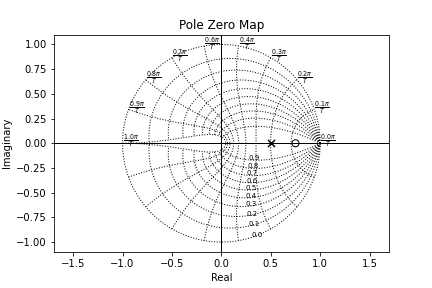
\includegraphics[width=\textwidth]{Img/3-euler.png}
            \caption{Diagrama de polos y ceros con metodo de Euler.}
            \label{fig:3-euler}
        \end{figure}

        \subsection{Adelanto}

        Para discretizar con diferencias por adelanto, debemos tomar la transformación 

        \begin{equation}
            s = \frac{z - 1}{hz} = \frac{ 4(z-1) }{z}
        \end{equation}

        Por lo tanto tenemos 

        \begin{equation}
            H(z) = \frac{4( 4z - 4 + z )}{4z -4 + 2z} = \frac{4( 5z - 4 )}{6z - 4}
        \end{equation}

        El diagrama de polos y ceros se puede observar en la figura \ref{fig:3-adelanto}.

        \begin{figure}[!htb]
            \centering
            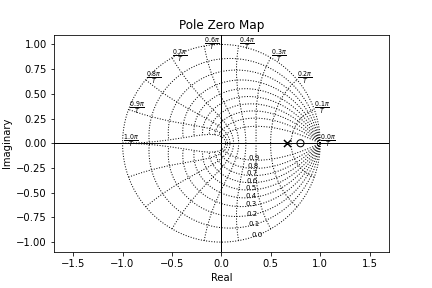
\includegraphics[width=\textwidth]{Img/3-adelanto.png}
            \caption{Diagrama de polos y ceros con diferencias por adelanto.}
            \label{fig:3-adelanto}
        \end{figure}

        \subsection{Tustin}

        Para discretizar un sistema por el metodo de Tustin debemos utilizar la transformacion 

        \begin{equation}
            s = \frac{ 2 }{h} \frac{z - 1}{z + 1} = 8 \frac{z - 1}{z + 1}
        \end{equation}

        Finalmente el sistema discretizado que se obtiene es 

        \begin{equation}
            H(z) = \frac{2( 9z - 7 )}{5z - 3}
        \end{equation}

        El diagrama de polos y ceros se observa en la figura \ref{fig:3-tustin}.

        \begin{figure}[!htb]
            \centering
            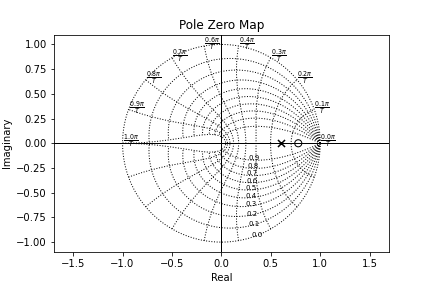
\includegraphics[width=\textwidth]{Img/3-tustin.png}
            \caption{Diagrama de polos y ceros discretizando con Tustin.}
            \label{fig:3-tustin}
        \end{figure}

    \section{Ejercicio 4}

    Para este ejercicio se utilizara un controlador PI continuo

    \begin{equation}
        G_c(s) = K\left( 1 + \frac{1}{T_i s} \right)
    \end{equation}

    \subsection{a)}

    Se utilizara la aproximación bilineal o de Tustin, con lo que se obtiene 
    
    \begin{equation}
        G_c(z) = \frac{K [ (K_i + 1 )z + ( K_i - 1 ) ] }{ z - 1 }, K_i = \frac{h}{2T_i}
    \end{equation}

    \subsection{b)}

    Se tiene que la transferencia del proceso es 

    \begin{equation}
        G_p(z) = \frac{z + 2}{z - 1/2}
    \end{equation}

    \begin{figure}[!htb]
        \centering
        \begin{tikzpicture}[node distance=2.5cm,auto,>=latex']
            \node [input, name=input] {};
            \node [sum, right of=input] (sum) {$+$};
            \node [block, right of=sum] (controller) {$G_c(z)$};
            \node [block, right of =controller, node distance=3.5cm] (system) { $G_p(z)$ };

            \draw [->] (controller) -- node[name=u] { $u$ } (system);
            \node [output, right of=system] (output) {};
            \node [output, below of=u] (H) {};
            
            \draw [draw, ->] (input) -- node {$r$} (sum); 
            \draw [->] (sum) -- node {$e$} (controller);
            \draw [->] (system) -- node[name=y] {$y$} (output);
            \draw [-] (y) |- (H);    
            \draw [->] (H) -| node[pos=0.99] {$-$} (sum);

        \end{tikzpicture}
        \caption{Diagrama en bloques del sistema}
        \label{}
    \end{figure}

    En este caso como el controlador discretizado tiene un polo en $1$ se puede comprobar que el error en estado estacionario 
    para una entrada escalon es nulo. Para determinar $K$ y $K_i$ se plantea el polinomia caracterisco $P(z)$ el cual es de la forma 

    \begin{equation}
        P(z) = z^2 + \underbrace{\left( KK_i + K - \frac{3}{2} \right)}_{b} z + \underbrace{\left( KK_i - K + \frac{1}{2} \right)}_{c}
    \end{equation}

    Por lo tanto los ceros del sistema retroalimentado se encuentran en 

    \begin{equation}
        z_{1,2} = -\frac{b}{2} \pm \frac{1}{2} \sqrt{ \underbrace{ b^2 - 4c }_{\Delta} }
    \end{equation}

    Por simplicidad en los calculos tomaremos 

    \begin{equation}
        \Delta = 0 \land \left\| \frac{b}{2} \right\| < 1
    \end{equation}

    Por otro lado fijaremos los polos en $-1/4$, teniendo entonces 

    \begin{equation}
        \frac{b}{2} = \frac{1}{4}
    \end{equation}

    Si llamamos $K_i^\prime = K K_i$ entonces despejando de la ecuación anterior, se tiene

    \begin{equation}
        K_i^\prime = 2 - K
    \end{equation}

    Si planteamos $\Delta = 0$ 

    \begin{equation}
        \left( K_i^\prime + K - \frac{3}{2} \right)^2 - 4 \left( K_i^\prime - K + \frac{1}{2} \right) = 0
    \end{equation}

    Remplazando $K_i^\prime$

    \begin{equation}
        \left( 2 - \frac{3}{2} \right)^2 - 4 \left( 2 - 2K + \frac{1}{2} \right) = 0
    \end{equation}

    Al despejar se obtiene 

    \begin{equation}
        K = \frac{23}{32} \land K_i = \frac{41}{23}
    \end{equation}

    Con lo que obtenemos un sistema estable y causal, con polos en $-1/4$.

    \section{Ejercicio 5}

    \begin{figure}[!htb]
        \centering
        \begin{tikzpicture}[node distance=3cm,auto,>=latex']
            \node [input] (input) {};
            \node [block, right of=input] (DAC) {DAC};
            \node [block, right of=DAC] (process) {$G_p(s)$};
            \node [block, right of= process] (ADC) {ADC};

            \draw [->] (DAC) -- node[yshift=1cm] {
                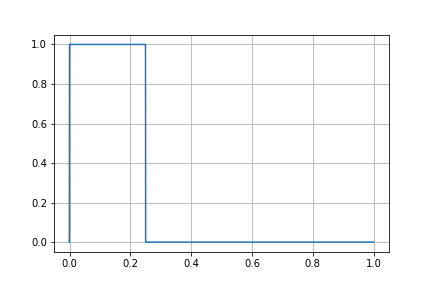
\includegraphics[width=3cm]{Img/5-DAC.png}
            } (process);

            \node [output, right of=ADC] (output) {};
            
            \draw [draw, ->] (input) -- node[yshift=1cm] {
                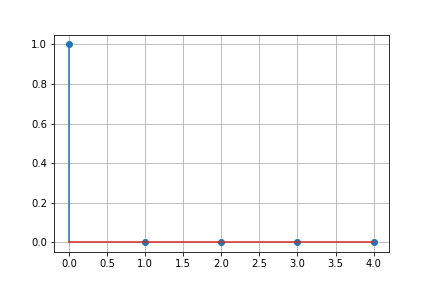
\includegraphics[width=3cm]{Img/5-input.png}
            } (DAC);

            \draw [->] (process) -- node[yshift=1cm] {
                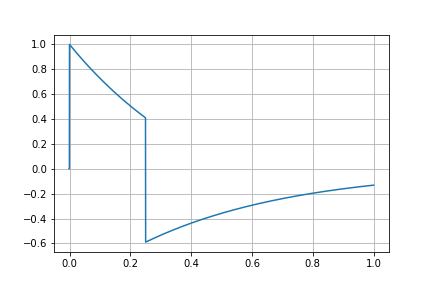
\includegraphics[width=3cm]{Img/5-G-P.png}
            } (ADC);

            \draw [->] (ADC) -- node[yshift=1cm] {
                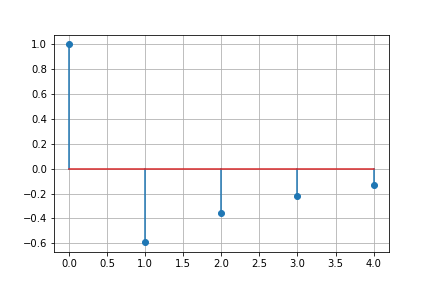
\includegraphics[width=3cm]{Img/5-G-P-D.png}
            } (output);
        \end{tikzpicture}
        \caption{Representación del mantenedor de orden cero.}
        \label{}
    \end{figure}

    Es posible generalizar el proceso mediante la siguiente formula 

    \begin{equation}
        \label{eq:ZOH}
        G_p(z) = (1 - z^{-1}) \textbf{Z} \left[ \textbf{L}^{-1} \left\{ \frac{G_p(s)}{s}  \right\}_{t=hk}  \right]
    \end{equation}

    En este caso $G_p(s)$ se escribe como 

    \begin{equation}
        G_p(s) = \frac{s-1}{s+2}
    \end{equation}

    Por lo tanto 

    \begin{equation}
        \frac{G_p(s)}{s} = \frac{s-1}{s(s+2)} = \frac{A}{s} + \frac{B}{s+2}
    \end{equation}

    Resolviendo las fracciones simples tenemos 

    \begin{equation}
        \frac{G_p(s)}{s} = \frac{3}{2s + 4} - \frac{1}{2s}
    \end{equation}

    Por lo que su transformada inversa de Laplace es 

    \begin{equation}
        p(t) = \left[ \frac{3}{2} e^{-2t} - \frac{1}{2} \right] \mu(t) 
    \end{equation}

    Al discretizar $p(t)$ se tiene que 

    \begin{equation}
        p[k] = \frac{1}{2} \left\{ 3 e^{-2hk} - 1  \right\} \mu[k]
    \end{equation}

    Al aplicar la transformada $Z$ a $p[k]$ 

    \begin{equation}
        P(z) = \frac{1}{2} \left\{ \frac{3}{1 - e^{-2h}z^{-1}} - \frac{1}{1 - z^{-1}} \right\}
    \end{equation}

    Finalmente para obtener la transferencia discretizada 

    \begin{equation}
        G(z) = (1 - z^{-1}) P(z) = \frac{1}{2} \left\{ \frac{3(1 - z^{-1})}{1 - e^{-2h}z^{-1}} - 1 \right\}
    \end{equation}

    \begin{equation}
        G(z) = \frac{2 + ( e^{-2h} - 3 )z^{-1}}{2( 1 - e^{-2h}z^{-1} )}
    \end{equation}

    \subsection{Respuesta al escalon}

    Para comparar la respues al escalon, podemos observar que en la ecuación \ref{eq:ZOH} se realiza la 
    transformada inversa de $G(s)/s$ es decir la respuesta al escalon del sistema continuo, por lo tanto 
    la respuesta al escalon del sistema continuo es $p(t)$. Por otro lado si al sistema discreto se le 
    introduce tenemos 

    \begin{equation}
        p[k] = \textbf{Z}^{-1} \left[ \frac{1}{1-z^{-1}}G_p(z) \right]
    \end{equation}

    Utilizando la expresión de la ecuación \ref{eq:ZOH}

    \begin{equation}
        p[k] = \textbf{Z}^{-1} \left\{ \frac{1}{1-z^{-1}} (1 - z^{-1}) \textbf{Z} \left[ \textbf{L}^{-1} \left( \frac{G_p(s)}{s}  \right)_{t=hk}  \right]  \right\}
    \end{equation}

    De la ecuacion anterior se puede pasar a 

    \begin{equation}
        p[k] = \textbf{Z}^{-1} \left\{  \textbf{Z} \left[ \textbf{L}^{-1} \left( \frac{G_p(s)}{s}  \right)_{t=hk}  \right]  \right\}
    \end{equation}

    Por lo que es trivial que 

    \begin{equation}
        p[k] = p(t)|_{t=hk}
    \end{equation}

    Y por lo tanto $p[k]$ es una versión muestreada de $p(t)$ con un periodo $h$.

    \section{Ejercicio 6}

        Para este ejercicio se tiene que 

        \begin{equation}
            A = \begin{bmatrix}
                    -0.2 & 0 \\
                    0.18 & -0.13 
                \end{bmatrix}
            \land 
            B = \begin{bmatrix}
                    0.26 \\    
                    0
                \end{bmatrix}
            \land 
            C = \begin{bmatrix}
                    1 & 0
                \end{bmatrix}
        \end{equation}

        La transferencia del proceso es 

        \begin{equation}
            G_p(s) = C(sI-A)^{-1}B
        \end{equation}

        En este caso 

        \begin{equation}
            G_p(s) = \frac{117/2500}{(s+0.2)(s+0.13)}
        \end{equation}

        \subsection{a)}

        \begin{equation}
            G_c(s) = K \left( 1 + \frac{1}{T_i s} \right)
        \end{equation}

        Ajustaremos un controlador PI, los criterios a cumplir son 

        \begin{itemize}
            \item Error en estado estacionario nulo para una entrada escalon
            \item $\omega_x=0.25 rad/s$
            \item $MF=50^\circ$
        \end{itemize}

        \subsubsection{Error nulo en estado estacionario}

        Al ser un controlador PI el error es nulo para una entrada escalon.

        \subsubsection{Ajustar $T_i$ para obtener $\omega_c=0.25rad/s$}

        Por condicion 

        \begin{equation}
            \arg( G(j\omega_x) )= -180^\circ
        \end{equation}

        Es posible plantear 

        \begin{equation}
            -\arg( j\omega_x + 0.2 ) - \arg( j\omega_x + 0.13 ) - \arg( j\omega_x ) + \arg( T_ij\omega_x + 1 ) + \arg( K ) = -180^{\circ}
        \end{equation}

        \begin{table}[H]
            \centering
            \begin{tabular}{|c|c|}
                \hline & $\arg [^\circ]$ \\ 
                \hline $j\omega_x + 0.2$ & $51.34$ \\
                \hline $j\omega_x + 0.13$ & $62.52$ \\
                \hline $j\omega_x$ & $90$ \\
                \hline $K$ & $0$ \\
                \hline
            \end{tabular}
            \caption{Aporte de fase en $\omega_x=0.25rad/seg$ tomando $K>0$.}
        \end{table}

        Por lo tanto 

        \begin{equation}
            \arctan{ T_i \omega_x } = 23.86^\circ
        \end{equation}

        Finalmente 

        \begin{equation}
            T_i = 1.77
        \end{equation}

        \subsubsection{Ajustar $K$ para obtener el margen de fase requerido}

        Para tener un margen de fase de $30^\circ$ el sistema en lazo abierto debe tener 

        \begin{equation}
            \arg(G(j\omega_c)) = -130^{\circ}
        \end{equation}

        Como hipotesis tomaremos que $\arg( T_ij\omega_c + 1 )\approx 0$ y luego lo verificaremos. Entonces el 
        argumento del sistema se puede plantear como 

        \begin{equation}
           \underbrace{\arg( T_ij\omega_c + 1 )}_{0} - \arg( (j\omega_c)^2 +0.2j\omega_c + 0.13j\omega_c + 0.026 ) - \underbrace{\arg(j\omega_c)}_{90^\circ} = -130^\circ
        \end{equation}

        Simplificando la ecuación anterior 

        \begin{equation}
            \frac{0.33\omega_c}{ 0.026 - \omega_c^2 } = \tan{-40^\circ}
        \end{equation}

        Despejando se obtiene la siguiente ecuacón 

        \begin{equation}
            -0.84\omega_c^2 - 0.33\omega_c + 0.02 = 0
        \end{equation}

        Cuyas raices son 

        \begin{equation}
            \omega_c \in \{ 0.053 , -0.45  \}
        \end{equation}

        Por lo tanto $\omega_c = 0.053rad/s$.

        Ahora el valor de $K$ debe ser tan que $|G(j\omega_c)|=1$ entonces 

        \begin{equation}
            K = \frac{1}{|G(j\omega_c)|} = 0.058        
        \end{equation}

        \subsubsection{Verificación}

        Para verificar la hipotesis calculamos el argumento de $T_ij\omega_c+1$.

        \begin{equation}
            \arctan{ T_i\omega_c } = 0.09r = 5.35^\circ
        \end{equation}

        Por lo tanto la aproximación es correcta.

        \subsection{b)}

            La transferencia de la planta retroalimentada es 

            \begin{equation}
                H(s) = \frac{AK( T_i s + 1 )}{ T_is( s + 0.2 )(s + 0.13) + AK(T_i s + 1) }
            \end{equation}

            Cuyos polos se encuentran en 

            \begin{equation}
                p_i \in \{ -0.23, -0.047+0.06j, -0.047-0.06j  \}
            \end{equation}

        \subsection{c)}

            Para discretizar el controlador utilizaremos el metodo de Euler

            \begin{equation}
                s = \frac{z-1}{h}
            \end{equation}

            Por lo tanto

            \begin{equation}
                G_c(z) = K\left( 1 + \frac{h^\prime}{z-1} \right), h^\prime = \frac{h}{T_i}
            \end{equation}

            Finalmente 

            \begin{equation}
                G_c(z) = K \frac{ z + ( h^\prime - 1 ) }{z - 1}
            \end{equation}

    \section{Ejercicio 7}

        Para el controlador PID fisicamente realizable 

        \begin{equation}
            G(s) = K\left( 1 + \frac{1}{T_is} + \frac{T_ds}{1 + T_ds/N} \right), N \geq 20
        \end{equation}

        Para el parte del integrador utilizaremos Euler y para la parte diferencia utilizaremos por adelanto 

        \begin{equation}
            s_{integrador} = \frac{z-1}{h} \land s_{derivador} = \frac{z-1}{zh}
        \end{equation}

        Por lo tanto se obtiene 

        \begin{equation}
            G(z) = K \left( 1 + \frac{h^\prime}{z-1} + \frac{T_d(z-1)}{[ hz + T_d(z-1)/N]} \right), h^\prime = \frac{h}{T_i}
        \end{equation}

        Simplificando 

        \begin{equation}
            G(z) = K \left( 1 +  \frac{h^\prime}{z-1} + \frac{T_d (z-1)}{ (h + T_d/N)z - T_d/N }   \right)
        \end{equation}
\end{document}